\documentclass[aspectratio=169,10pt]{beamer}
\usetheme{Madrid}
\usecolortheme{default}

\usepackage{hyperref}
\usepackage{tikz}
\usetikzlibrary{patterns,shapes,arrows,calc,positioning,decorations.markings}
\usepackage{circuitikz}
\usepackage{amsmath,amssymb}
\usepackage{graphicx}
\usepackage{listings}
\usepackage{booktabs}

% --- Custom Colors UNIB ---
\definecolor{unibblue}{RGB}{0, 32, 96}
\definecolor{unibgold}{RGB}{197, 160, 89}
\definecolor{unibgreen}{RGB}{34, 112, 60}

\setbeamercolor{palette primary}{bg=unibblue,fg=white}
\setbeamercolor{palette secondary}{bg=unibblue!85,fg=white}
\setbeamercolor{palette tertiary}{bg=unibblue!70,fg=white}
\setbeamercolor{structure}{fg=unibblue}
\setbeamercolor{titlelike}{parent=structure,bg=unibblue,fg=white}
\setbeamercolor{block title}{bg=unibblue!90,fg=white}
\setbeamercolor{block body}{bg=unibblue!8,fg=black}
\setbeamercolor{alertblock title}{bg=unibgold!95,fg=black}
\setbeamercolor{alertblock body}{bg=unibgold!15,fg=black}
\setbeamercolor{exampleblock title}{bg=unibgreen!90,fg=white}
\setbeamercolor{exampleblock body}{bg=unibgreen!10,fg=black}

% --- Pengaturan Listing Julia ---
\lstdefinelanguage{Julia}%
  {morekeywords={abstract,break,case,catch,const,continue,do,else,elseif,%
      end,export,false,for,function,global,if,import,%
      let,local,macro,module,mutable,primitive,quote,return,struct,%
      true,try,type,using,var,while},%
   sensitive=true,%
   morecomment=[l]{\#},%
   morecomment=[n]{\#=}{=\#},%
   morestring=[b]',%
   morestring=[b]"%
  }[keywords,comments,strings]

\lstdefinestyle{juliastyle}{
    language=Julia,
    basicstyle=\ttfamily\tiny,
    keywordstyle=\color{blue!80!black}\bfseries,
    commentstyle=\color{green!50!black}\itshape,
    stringstyle=\color{red!80!black},
    numbers=none,
    breaklines=true,
    showstringspaces=false,
    frame=single,
    backgroundcolor=\color{gray!6},
    xleftmargin=4pt,
    xrightmargin=4pt,
    aboveskip=2pt,
    belowskip=2pt
}

\title[Persamaan Diferensial (Minggu 5)]{Persamaan Diferensial}
\subtitle{Minggu 5: PDB Orde 2 Non-Homogen, Resonansi Frekuensi, \& RLC AC}
\author[Novalio \& Arfan (UNIB)]{Ir. Novalio Daratha, S.T., M.Sc., Ph.D. \& Muhammad Arfan, S.T., M.T.}
\institute[Teknik Elektro UNIB]{Program Studi S1 Teknik Elektro, Jurusan Teknik Elektro \& Informatika\\Fakultas Teknik, Universitas Bengkulu}
\date[2026]{Semester Genap 2026}

\begin{document}

% FRAME 1: Titlepage
\begin{frame}[plain]
  \titlepage
\end{frame}

% FRAME 2: Sub-CPMK OBE Bloom
\begin{frame}{Capaian Pembelajaran (Sub-CPMK 3) \& Taksonomi Bloom}
  \begin{block}{Sub-CPMK Minggu 5 (Sistem Tereksitasi Sumber Luar \& Resonansi AC)}
    Mahasiswa mampu memecahkan PDB linier orde 2 non-homogen menggunakan metode koefisien tak tentu, menganalisis respon transien dan keadaan mantap sirkuit RLC seri AC, serta mengevaluasi bahaya lonjakan tegangan resonansi dan fenomena beat.
  \end{block}
  \vspace{0.15cm}
  \begin{columns}[t]
    \column{0.5\textwidth}
    \textbf{Target Kognitif (Bloom C1--C3):}
    \begin{itemize}
      \item \textbf{C1 (Mengingat):} Menyatakan struktur solusi superposisi $y(t) = y_h(t) + y_p(t)$ dan aturan modifikasi $x^s$.
      \item \textbf{C2 (Memahami):} Membedakan respon alami yang meluruh vs respon paksa yang berosilasi tunak.
      \item \textbf{C3 (Menerapkan):} Menghitung solusi partikular $y_p(t)$ eksitasi sinusoidal $V_m \cos(\omega t)$.
    \end{itemize}

    \column{0.5\textwidth}
    \textbf{Target Kognitif (Bloom C4--C6):}
    \begin{itemize}
      \item \textbf{C4 (Menganalisis):} Menghitung faktor kualitas $Q$, impedansi $Z$, dan amplifikasi tegangan kapasitor.
      \item \textbf{C5 (Mengevaluasi):} Mengevaluasi dampak Resonansi Sub-Sinkron (SSR) pada poros turbin PLN.
      \item \textbf{C6 (Komputasi):} Memprogram kurva respon frekuensi dan modulasi layangan (\textit{beats}) dengan Julia.
    \end{itemize}
  \end{columns}
\end{frame}

% FRAME 3: Peta Konsep Solusi Superposisi
\begin{frame}{Peta Konsep: Struktur Solusi Lengkap Sistem Non-Homogen}
  \begin{block}{Teorema Dekomposisi Solusi PDB Non-Homogen}
    Untuk persamaan linier tak homogen $a y'' + b y' + c y = g(t)$, solusi lengkapnya merupakan penjumlahan:
    \begin{equation}
      \mathbf{y(t) = y_h(t) + y_p(t)}
    \end{equation}
  \end{block}
  \vspace{0.1cm}
  \begin{columns}[t]
    \column{0.5\textwidth}
    \begin{exampleblock}{1. Solusi Homogen / Alami ($y_h$)}
      \begin{itemize}
        \item Menyelesaikan persamaan $a y'' + b y' + c y = 0$.
        \item Ditentukan oleh dinamika internal ($R, L, C$).
        \item Selalu memuat faktor peluruhan $e^{-\alpha t}$ $\rightarrow$ \textbf{Respon Transien} ($y_h \to 0$ saat $t \to \infty$).
      \end{itemize}
    \end{exampleblock}

    \column{0.5\textwidth}
    \begin{alertblock}{2. Solusi Partikular / Paksa ($y_p$)}
      \begin{itemize}
        \item Menyelesaikan suku penggerak luar $g(t)$.
        \item Mengikuti bentuk matematika sumber eksitasi.
        \item Tetap bertahan sepanjang waktu $\rightarrow$ \textbf{Respon Keadaan Mantap} (\textit{Steady-State Response}).
      \end{itemize}
    \end{alertblock}
  \end{columns}
\end{frame}

% FRAME 4: Metode Koefisien Tak Tentu
\begin{frame}{Metode Koefisien Tak Tentu (\textit{Undetermined Coefficients})}
  Metode ini digunakan bila fungsi pendorong luar $g(t)$ berupa kombinasi fungsi dasar:
  \vspace{0.15cm}
  \begin{center}
    \small
    \begin{tabular}{ll}
      \toprule
      \textbf{Bentuk Fungsi Pendorong $g(t)$} & \textbf{Bentuk Tebakan Solusi Partikular $y_p(t)$} \\ \midrule
      Polinomial: $P_n(t) = a_n t^n + \dots + a_0$ & $A_n t^n + A_{n-1} t^{n-1} + \dots + A_0$ \\
      Eksponensial: $e^{k t}$ & $A e^{k t}$ \\
      Sinusoidal: $\cos(\omega t)$ atau $\sin(\omega t)$ & $A \cos(\omega t) + B \sin(\omega t)$ \\
      Campuran: $e^{k t} \cos(\omega t)$ & $e^{k t} [A \cos(\omega t) + B \sin(\omega t)]$ \\ \bottomrule
    \end{tabular}
  \end{center}
  \vspace{0.2cm}
  \footnotesize Koefisien konstanta $A, B$ ditentukan dengan menyubstitusikan $y_p, y_p', y_p''$ ke dalam PDB semula dan menyamakan koefisien aljabar pada kedua ruas.
\end{frame}

% FRAME 5: Aturan Modifikasi Resonansi x^s
\begin{frame}{Aturan Modifikasi Resonansi: Pengali $t^s$}
  \begin{alertblock}{Konflik Resonansi Aljabar}
    Jika tebakan awal $y_p(t)$ ternyata merupakan salah satu solusi dari persamaan homogen $y_h(t)$, maka substitusi $y_p$ ke ruas kiri akan menghasilkan \textbf{nol} ($0 = g(t)$, kontradiksi!).
  \end{alertblock}
  \vspace{0.15cm}
  \begin{block}{Aturan Pengali d'Alembert ($t^s$)}
    Kalikan tebakan awal $y_p(t)$ dengan $t^s$, di mana $s$ adalah bilangan bulat terkecil ($s=1$ atau $s=2$) yang menjamin tidak ada satupun suku dalam $y_p(t)$ yang menduplikasi suku dalam $y_h(t)$:
    \begin{itemize}
      \item $s = 1$: Jika frekuensi sumber luar $\omega$ sama dengan frekuensi alami $\omega_0$ pada sistem teredam kritis atau tak teredam.
      \item $s = 2$: Jika akar karakteristik kembar dan identik dengan eksitasi.
    \end{itemize}
    \textbf{Makna Fisik:} Menghasilkan amplifikasi amplitudo secara linier terhadap waktu ($t \sin\omega t$), yang merupakan ciri utama fenomena \textbf{Resonansi Murni}.
  \end{block}
\end{frame}

% FRAME 6: Pemodelan Sirkuit RLC AC dengan CircuiTikZ
\begin{frame}{Pemodelan Fisis: Sirkuit RLC Seri Eksitasi AC}
  \begin{columns}
    \column{0.45\textwidth}
    \begin{center}
      \resizebox{\linewidth}{!}{%
      \begin{circuitikz}[american, scale=1.1]
        \draw (0,0) to[sV, l=$v_s(t)$] (0,2.5)
              to[R, l=$R$, v=$v_R$] (2.0,2.5)
              to[L, l=$L$, v=$v_L$] (3.8,2.5)
              to[C, l=$C$, v=$v_C$] (3.8,0)
              -- (0,0);
        \draw[->, >=stealth, thick, unibblue] (1.9,1.2) arc (160:-160:0.6);
        \node at (2.5,1.2) [unibblue, font=\small\bfseries] {$i(t)$};
      \end{circuitikz}%
      }
    \end{center}
    \vspace{-0.2cm}
    \begin{center}
      \footnotesize Sirkuit RLC Seri dengan Sumber Sinusoidal $v_s(t) = V_m \cos(\omega t)$.
    \end{center}

    \column{0.55\textwidth}
    \textbf{Formulasi Hukum KVL Dinamis:}
    \begin{equation}
      v_R(t) + v_L(t) + v_C(t) = v_s(t)
    \end{equation}
    Dinyatakan dalam muatan kapasitor $q(t)$:
    \begin{equation}
      L \frac{d^2 q}{dt^2} + R \frac{dq}{dt} + \frac{1}{C} q = V_m \cos(\omega t)
    \end{equation}
    Atau diferensiasikan terhadap waktu untuk arus $i(t)$:
    \begin{block}{PDB Non-Homogen Arus RLC AC}
      \begin{equation*}
        \frac{d^2 i}{dt^2} + 2\alpha \frac{di}{dt} + \omega_0^2 i = -\frac{V_m \omega}{L} \sin(\omega t)
      \end{equation*}
    \end{block}
  \end{columns}
\end{frame}

% FRAME 7: Respon Transien vs Tunak
\begin{frame}{Evolusi Gelombang: Respon Transien vs Keadaan Mantap}
  \begin{columns}[c]
    \column{0.55\textwidth}
    \begin{center}
      \resizebox{0.95\linewidth}{!}{%
      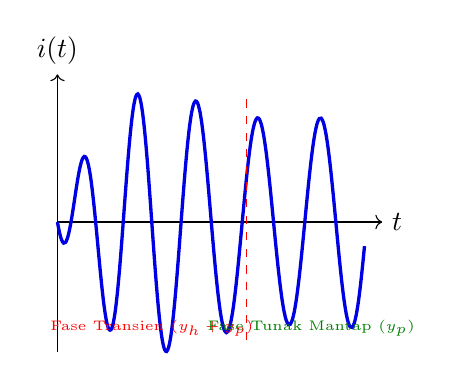
\begin{tikzpicture}[scale=0.75]
        \draw[->] (0,0) -- (5.5,0) node[right] {$t$};
        \draw[->] (0,-2.2) -- (0,2.5) node[above] {$i(t)$};
        % Kurva gabungan transien + tunak
        \draw[domain=0:5.2, samples=150, smooth, blue!90!black, very thick] plot ({\x}, {1.8*sin(6*\x r) - 2.2*exp(-0.9*\x)*sin(7.5*\x r)});
        % Garis batas transien
        \draw[dashed, red] (3.2,-2) -- (3.2,2.2);
        \node[red, font=\tiny] at (1.6,-1.8) {Fase Transien ($y_h + y_p$)};
        \node[green!50!black, font=\tiny] at (4.3,-1.8) {Fase Tunak Mantap ($y_p$)};
      \end{tikzpicture}%
      }
    \end{center}

    \column{0.45\textwidth}
    \begin{block}{Dinamika Gelombang}
      \begin{itemize}
        \item Pada awal pensaklaran ($t < 5\tau$), gelombang mengalami distorsi asimetris akibat komponen transien $y_h(t)$.
        \item Setelah $t \ge 5\tau$, komponen $y_h(t)$ lenyap sempurna ($e^{-\alpha t} \to 0$).
        \item Sistem memasuki \textbf{keadaan mantap harmonik murni} dengan frekuensi sumber $\omega$.
      \end{itemize}
    \end{block}
  \end{columns}
\end{frame}

% FRAME 8: Resonansi Seri & Faktor-Q
\begin{frame}{Resonansi Seri \& Pelipatgandaan Tegangan Reaktif Faktor-$Q$}
  \begin{columns}[c]
    \column{0.52\textwidth}
    \textbf{Kondisi Resonansi Seri:}
    \begin{itemize}
      \item Terjadi saat reaktansi induktif saling meniadakan reaktansi kapasitif:
      \begin{equation*}
        X_L = X_C \implies \omega L = \frac{1}{\omega C} \implies \mathbf{\omega_0 = \frac{1}{\sqrt{LC}}}
      \end{equation*}
      \item Impedansi total sirkuit mencapai titik minimum:
      \begin{equation*}
        \mathbf{Z_{\text{min}} = R}
      \end{equation*}
      \item Arus mencapai nilai maksimum: $I_{\text{maks}} = \frac{V_m}{R}$.
    \end{itemize}

    \column{0.44\textwidth}
    \begin{alertblock}{Bahaya Pelipatgandaan Tegangan}
      Tegangan reaktif kapasitor dan induktor saat resonansi:
      \begin{equation*}
        V_{C, \text{maks}} = I_{\text{maks}} X_C = \frac{V_m}{R} \frac{1}{\omega_0 C} = \mathbf{Q \cdot V_m}
      \end{equation*}
      dengan \textbf{Faktor Kualitas}:
      \begin{equation*}
        \mathbf{Q = \frac{\omega_0 L}{R} = \frac{1}{R}\sqrt{\frac{L}{C}}}
      \end{equation*}
      Bila $Q = 10$, tegangan melonjak $10\times$ lipat tegangan sumber!
    \end{alertblock}
  \end{columns}
\end{frame}

% FRAME 9: Fenomena Beat
\begin{frame}{Fenomena Denyut Layangan (\textit{Beat Phenomenon}, $\omega \approx \omega_0$)}
  \begin{columns}[c]
    \column{0.55\textwidth}
    Jika $R \approx 0$ dan frekuensi eksitasi $\omega \approx \omega_0$:
    \begin{equation*}
      q(t) = \frac{2 V_m}{L(\omega_0^2 - \omega^2)} \sin(\omega_{\text{mod}} t) \sin(\omega_{\text{carrier}} t)
    \end{equation*}
    \begin{itemize}
      \item \textbf{Gelombang Pembawa:} $\omega_{\text{carrier}} = \frac{\omega_0 + \omega}{2} \approx \omega_0$.
      \item \textbf{Selubung Modulasi:} $\omega_{\text{mod}} = \frac{|\omega_0 - \omega|}{2}$.
      \item \textbf{Frekuensi Denyut Layangan (\textit{Beat}):}
      \begin{equation*}
        \mathbf{f_{\text{beat}} = \frac{|\omega_0 - \omega|}{2\pi}} \quad [\text{Hz}]
      \end{equation*}
    \end{itemize}

    \column{0.45\textwidth}
    \begin{center}
      \resizebox{!}{0.55\textheight}{%
      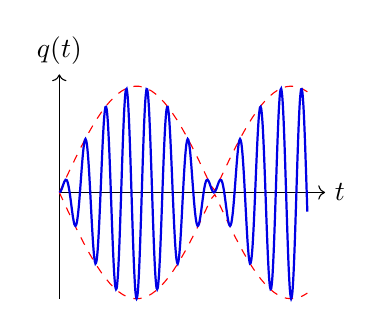
\begin{tikzpicture}[scale=0.75]
        \draw[->] (0,0) -- (4.5,0) node[right] {$t$};
        \draw[->] (0,-1.8) -- (0,2.0) node[above] {$q(t)$};
        % Selubung beat
        \draw[dashed, red] plot[domain=0:4.2, samples=60] ({\x}, {1.8*abs(sin(1.2*\x r))});
        \draw[dashed, red] plot[domain=0:4.2, samples=60] ({\x}, {-1.8*abs(sin(1.2*\x r))});
        % Gelombang beat
        \draw[domain=0:4.2, samples=200, smooth, blue!90!black, thick] plot ({\x}, {1.8*sin(1.2*\x r)*sin(18*\x r)});
      \end{tikzpicture}%
      }
    \end{center}
  \end{columns}
\end{frame}

% FRAME 10: Resonansi Sub-Sinkron PLN
\begin{frame}{Studi Kasus Industri: Resonansi Sub-Sinkron (SSR) PLN}
  \begin{columns}[c]
    \column{0.55\textwidth}
    \textbf{Fenomena Resonansi Torsi Sub-Sinkron (SSR):}
    \begin{itemize}
      \item Pada saluran transmisi daya EHV 500 kV yang dilengkapi kapasitor bank kompensasi seri, terbentuk frekuensi resonansi alami sub-sinkron $f_{\text{er}} < 50\text{ Hz}$ (biasanya $20\text{ s.d. } 45\text{ Hz}$).
      \item Jika frekuensi komplemen $f_m = 50\text{ Hz} - f_{\text{er}}$ bertepatan dengan salah satu moda getaran mekanis torsional poros turbin-generator:
      \begin{equation*}
        \mathbf{f_{\text{torsi}} \approx 50\text{ Hz} - f_{\text{er}}}
      \end{equation*}
      \item Terjadi amplifikasi torsi osilatif destruktif yang dapat mematahkan poros turbin generator pembangkit!
    \end{itemize}

    \column{0.45\textwidth}
    \begin{alertblock}{Standar IEEE Std 775}
      Transmisi terkompensasi seri wajib dilengkapi relai proteksi SSR (\textit{Subsynchronous Damping Scheme}) dan filter aktif fleksibel (FACTS/TCSC) untuk menjamin redaman positif pada seluruh rentang frekuensi sub-sinkron.
    \end{alertblock}
  \end{columns}
\end{frame}

% FRAME 11: Worked Example 1 - Resonansi RLC
\begin{frame}{Contoh Soal 1 (Worked Example): Resonansi Tegangan RLC}
  \textbf{Kasus RLC AC:} Parameter $R = 10\,\Omega$, $L = 0{,}1\text{ H}$, $C = 10\,\mu\text{F}$ disuplai generator $v_s(t) = 100 \cos(\omega t)\text{ V}$.
  \vspace{0.15cm}

  \begin{columns}[t]
    \column{0.5\textwidth}
    \textbf{1. Frekuensi Resonansi \& Faktor-$Q$:}
    \begin{align*}
      \omega_0 &= \frac{1}{\sqrt{LC}} = \frac{1}{\sqrt{0{,}1 \times 10\mu\text{F}}} = \mathbf{1000\text{ rad/s}} \\
      Q &= \frac{\omega_0 L}{R} = \frac{1000 \times 0{,}1}{10} = \mathbf{10}
    \end{align*}
    \textbf{2. Pada Resonansi ($\omega = 1000\text{ rad/s}$):}
    \begin{align*}
      Z &= R = 10\,\Omega \implies I_{\text{maks}} = \frac{100\text{ V}}{10\,\Omega} = \mathbf{10\text{ A}} \\
      \mathbf{i(t)} &= \mathbf{10 \cos(1000 t)\quad [\text{Ampere}]}
    \end{align*}

    \column{0.5\textwidth}
    \textbf{3. Lonjakan Tegangan Kapasitor ($V_C$):}
    \begin{equation*}
      V_{C, \text{maks}} = Q \times V_m = 10 \times 100\text{ V} = \mathbf{1000\text{ Volt!}}
    \end{equation*}
    Isolasi kapasitor harus dirancang mampu menahan tegangan $10\times$ lebih tinggi dari suplai!
    \vspace{0.15cm}

    \textbf{4. Pada Kondisi Off-Resonansi ($\omega = 500\text{ rad/s}$):}
    \begin{align*}
      X_L &= 500(0{,}1) = 50\,\Omega, \quad X_C = \frac{1}{500(10\mu\text{F})} = 200\,\Omega \\
      Z &= \sqrt{10^2 + (50 - 200)^2} = \mathbf{150{,}3\ \Omega} \\
      I_m &= \frac{100}{150{,}3} = \mathbf{0{,}665\text{ A}} \quad (\text{Drop }>93\%)
    \end{align*}
  \end{columns}
\end{frame}

% FRAME 12: Worked Example 2 - Fenomena Beat SSR
\begin{frame}{Contoh Soal 2 (Worked Example): Denyut Layangan SSR}
  \textbf{Kasus Transmisi Terkompensasi:} Persamaan muatan $q'' + 314^2 q = 100 \cos(300 t)$ dengan kondisi awal $q(0)=0, q'(0)=0$ (frekuensi alami $\omega_0 = 314\text{ rad/s}$, eksitasi $\omega = 300\text{ rad/s}$).
  \vspace{0.15cm}

  \begin{columns}[t]
    \column{0.5\textwidth}
    \textbf{1. Frekuensi Denyut \& Pembawa:}
    \begin{align*}
      \omega_{\text{mod}} &= \frac{\omega_0 - \omega}{2} = \frac{314 - 300}{2} = \mathbf{7\text{ rad/s}} \\
      \omega_{\text{carrier}} &= \frac{\omega_0 + \omega}{2} = \frac{314 + 300}{2} = \mathbf{307\text{ rad/s}}
    \end{align*}
    \textbf{2. Amplitudo Puncak Layangan:}
    \begin{equation*}
      A_{\text{beat}} = \frac{2 \times 100}{314^2 - 300^2} = \frac{200}{8596} = \mathbf{0{,}0233\text{ C}}
    \end{equation*}

    \column{0.5\textwidth}
    \textbf{3. Persamaan Gelombang Lengkap:}
    \begin{equation*}
      \mathbf{q(t) = 0{,}0233 \sin(7 t) \sin(307 t)\quad [\text{Coulomb}]}
    \end{equation*}
    \textbf{4. Frekuensi Siklik Denyut Layangan:}
    \begin{equation*}
      f_{\text{beat}} = \frac{|\omega_0 - \omega|}{2\pi} = \frac{14}{2\pi} = \mathbf{2{,}23\text{ Hz}}
    \end{equation*}
    Poros mekanis turbin akan berdenyut dengan frekuensi $2{,}23\text{ Hz}$, memicu risiko patah kelelahan bahan (\textit{mechanical fatigue}).
  \end{columns}
\end{frame}

% FRAME 13: Praktikum Komputasi Julia
% FRAME 13: Praktikum Komputasi Julia
\begin{frame}[fragile]{Praktikum Komputasi Julia: Resonansi RLC \& Selektivitas}
  \begin{columns}[t]
    \column{0.50\textwidth}
    \begin{block}{Skrip Julia: Kurva Respon Frekuensi}
\begin{lstlisting}[style=juliastyle]
using Plots

w_w0 = range(0.5, 1.5, length=300)
H(w_ratio, Q) = 1.0 ./ sqrt.(1.0 .+ Q^2 .* (w_ratio .- 1.0 ./ w_ratio).^2)

plot(w_w0, H.(w_w0, 2), label="Q = 2", lw=2)
plot!(w_w0, H.(w_w0, 5), label="Q = 5", lw=2)
plot!(w_w0, H.(w_w0, 10), label="Q = 10", lw=2)
vline!([1.0], ls=:dash, label="Resonansi")
\end{lstlisting}
    \end{block}

    \column{0.48\textwidth}
    \begin{alertblock}{Visualisasi Resonansi \& $Q$}
      \centering
      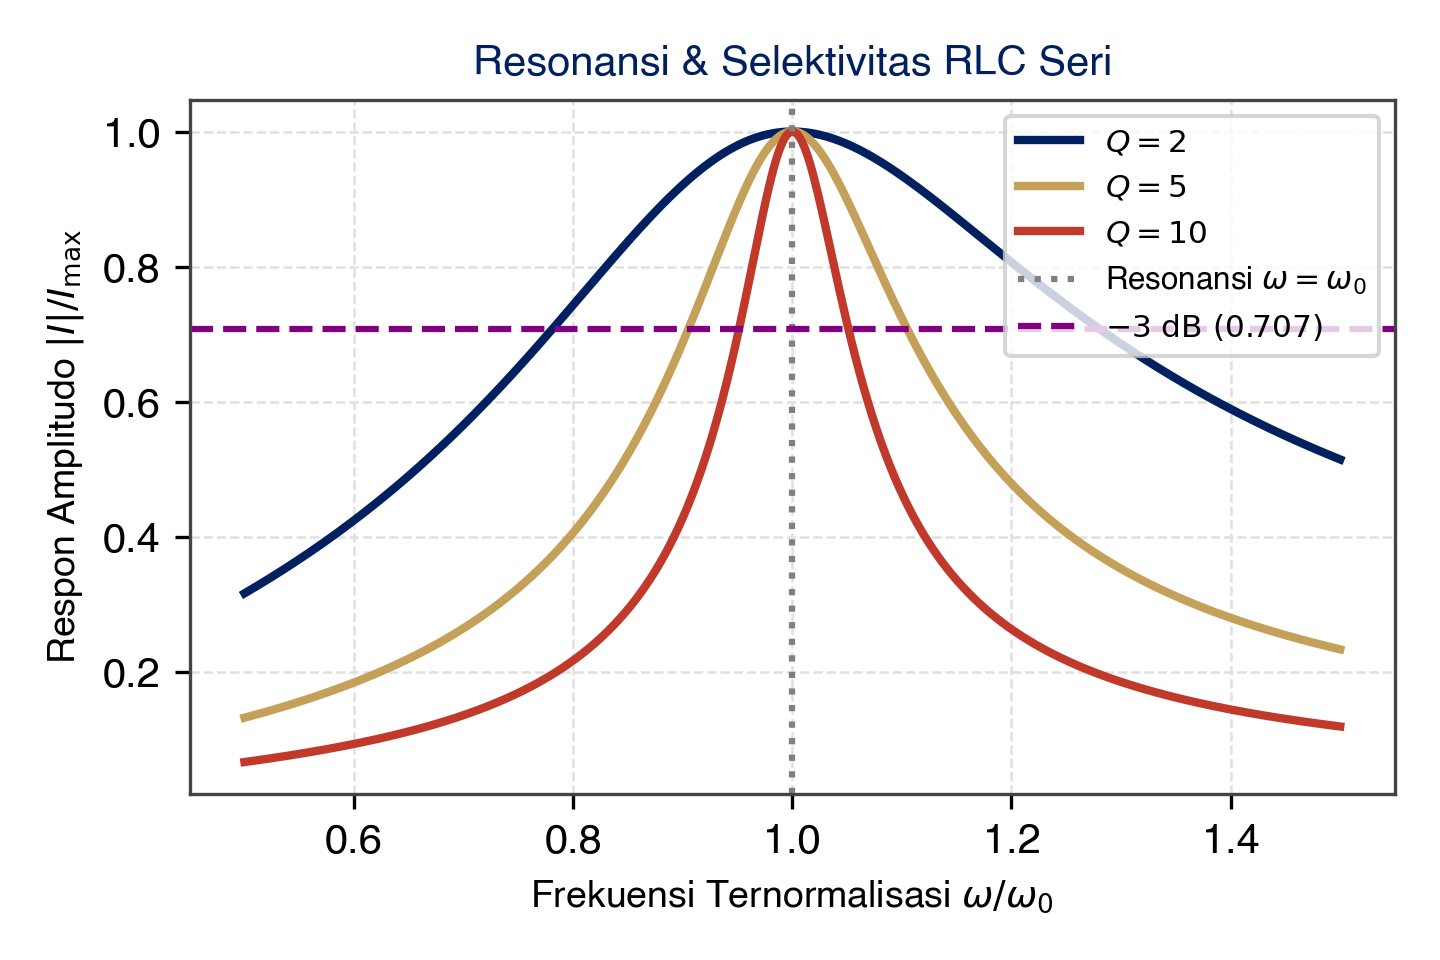
\includegraphics[width=\linewidth, height=0.38\textheight, keepaspectratio]{figures/slides/plot_ch5.png}
    \end{alertblock}
    \vspace{-0.1cm}
    \begin{exampleblock}{Intisari Resonansi}
      \tiny
      Saat $\omega = \omega_0$, reaktansi $X_L = X_C$, impedansi minimum $Z = R$. Nilai $Q$ tinggi mempertajam selektivitas kurva, namun memperbesar tegangan jatuh pada $L$ dan $C$ ($V_C = Q V_s$).
    \end{exampleblock}
  \end{columns}
\end{frame}

% FRAME 14: Kuis & Tantangan Bloom C1-C6
% FRAME 14: Kuis & Tantangan Bloom C1-C6
\begin{frame}{Kuis Konseptual Interaktif \& Evaluasi Bloom (C1--C6)}
  \begin{columns}[t]
    \column{0.52\textwidth}
    \begin{alertblock}{Peer Instruction: Uji Miskonsepsi Fisik}
      \footnotesize
      \textbf{Kasus Rekayasa:} RLC seri AC mengalami resonansi seri ($Q = 10$). Voltmeter mengukur tegangan kapasitor $V_C = 1000\text{ V}$ padahal sumber $V_s$ hanya $100\text{ V}$. Apakah ini melanggar hukum energi?
      \vspace{0.05cm}
      \begin{itemize}\setlength{\itemsep}{1pt}
        \item \textbf{[A]} Ya, tegangan komponen tidak boleh melebihi sumber.
        \item \textbf{[B]} **Tidak**, karena $V_C$ dan $V_L$ berbeda fasa $180^\circ$ sehingga saling meniadakan secara vektor total ($V_C + V_L = 0$)!
        \item \textbf{[C]} Ya, terjadi pembangkitan daya aktif tambahan.
        \item \textbf{[D]} Tidak, asalkan frekuensi sumber di atas $1\text{ kHz}$.
      \end{itemize}
    \end{alertblock}

    \column{0.46\textwidth}
    \begin{block}{Tantangan Analisis \& Desain (C4--C6)}
      \footnotesize
      \begin{itemize}\setlength{\itemsep}{2pt}
        \item \textbf{C4 (Analisis):} Analisis risiko Sub-Synchronous Resonance (SSR) pada poros turbin generator akibat kompensasi kapasitor seri.
        \item \textbf{C5 (Evaluasi):} Evaluasi bandwidth $-3\text{ dB}$ filter bandpass untuk menyaring harmonisa ke-5 PLN.
        \item \textbf{C6 (Desain):} Rancang parameter filter pasif RLC seri dengan $f_0 = 250\text{ Hz}$ dan $Q = 15$!
      \end{itemize}
    \end{block}
  \end{columns}
\end{frame}

% FRAME 15: Rangkuman & Penutup
\begin{frame}{Rangkuman Inti Perkuliahan \& Referensi}
  \begin{exampleblock}{Intisari Perkuliahan Minggu 5}
    \begin{itemize}
      \item Solusi PDB orde 2 non-homogen adalah superposisi respon transien $y_h(t)$ dan respon keadaan mantap $y_p(t)$.
      \item Pada resonansi seri ($\omega = \omega_0$), impedansi minimum ($Z = R$), arus maksimum, dan tegangan reaktif mengalami amplifikasi sebesar faktor-$Q$.
      \item Frekuensi eksitasi yang berdekatan dengan frekuensi alami menghasilkan denyut layangan (\textit{beats}) yang dapat memicu kegagalan mekanis pada turbin daya (SSR).
    \end{itemize}
  \end{exampleblock}
  \vspace{0.2cm}
  \begin{center}
    \small \textbf{Buku Acuan Utama:} \\
    E. Kreyszig, \textit{Advanced Engineering Mathematics} | W. Hayt, \textit{Engineering Circuit Analysis}. \\
    \vspace{0.3cm}
    \textbf{Tautan Modul \& Bahan Ajar}: \url{https://www.ndaratha.my.id/persamaan-diferensial/}
  \end{center}
\end{frame}

\end{document}
